
\section{Data}
The dataset\cite{KAGGLEDATA} consists of 17,500 aerial images out of which 13,136 contain an columnar cacti  and 4,364 do not.  Each image is 32x32 in size. The images have been resized by kaggle to be uniform in size. The dataset also contains an .csv file that annoates for each image if it contains an columnar cacti or not. The images are all from the Tehucan-Cuicatlan valley in the south of Mexico \cite{LOPEZJIMENEZ2019}. The images have been obtained using a drone from an flight altitude of 100 m. The images were manually labeled. The dataset also contains 4000 images for verification, 3000 of which are showing an cactus and 1000 are not.
\begin{figure}[h]
    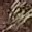
\includegraphics[width=.09\textwidth]{images/1.jpg}
     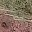
\includegraphics[width=.09\textwidth]{images/2.jpg}
    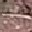
\includegraphics[width=.09\textwidth]{images/3.jpg}
    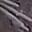
\includegraphics[width=.09\textwidth]{images/4.jpg}
    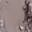
\includegraphics[width=.09\textwidth]{images/5.jpg}
    \caption{Example images from the dataset}
\end{figure}
